\chapter{基于定向探索模型的离线到在线强化学习算法}\label{Chap:chap4}

本章详细介绍本文提出的基于定向探索模型的离线到在线强化学习算法。首先分析现有方法的局限性并阐明算法设计动机；随后系统阐述算法的整体框架，包括离线预训练阶段和在线定向探索阶段；接着深入讨论不确定性估计方法与动态权重自适应机制；然后给出算法的理论分析，证明定向探索策略相比均匀采样具有更优的收敛速率；最后通过在D4RL基准测试集上的实验验证算法的有效性，并与现有方法进行系统对比。


\section{问题分析与算法动机}\label{Sec4.1}

如第二章所述，离线到在线强化学习面临的核心挑战在于如何平衡离线阶段的保守性与在线阶段的探索性。现有方法通常在离线阶段采用保守算法抑制分布外过估计，在在线阶段逐步放松约束以适应新数据。然而，这类方法存在以下根本性局限：

第一，保守性约束在在线阶段形成探索瓶颈。离线阶段学习的保守策略倾向于在低不确定性区域内采样，即使放松约束后，策略仍难以快速适应分布外区域。这导致在线采集的样本集中在离线数据已覆盖的区域，对转移模型的改进贡献有限。

第二，不确定性信息未得到充分利用。现有基于模型的方法主要将不确定性用于惩罚高不确定性区域的奖励，以避免策略访问模型预测不可靠的状态-动作对。这种被动利用方式忽视了不确定性信息的另一层含义：高不确定性区域恰恰对应模型泛化能力不足的区域，是在线探索应优先补充的目标。

第三，在线交互成本高昂。多数离线到在线方法为无模型方法，需要大量在线交互（通常需要200k步）才能实现有效微调。在实际应用中，与真实环境的每次交互都可能产生成本或风险，因此如何以最少的在线交互实现高效微调具有重要意义。

基于上述分析，本文提出将不确定性信息从"惩罚信号"转变为"探索引导信号"的核心思想。当采集在线样本时，策略应被引导至高不确定性（转移模型覆盖之外）且高动作价值（接近目标）的区域。高不确定性区域的样本可有效补充转移模型的训练数据，提升模型在全状态-动作空间的泛化能力；高动作价值区域的样本则确保采集的数据对策略优化有直接贡献，避免探索无关区域造成的资源浪费。这种定向探索策略将在线交互的信息增益最大化，以最少的交互次数实现高效微调。


\section{算法框架}\label{Sec4.2}

本文提出的基于定向探索模型的离线到在线强化学习算法采用两阶段框架：离线预训练阶段在静态数据集上学习转移模型和初始策略；在线微调阶段通过定向探索采集高价值样本，迭代更新模型和策略。算法的整体流程如图\ref{Fig:Chap4_framework}所示。

\begin{figure}[htbp]
  \centering
  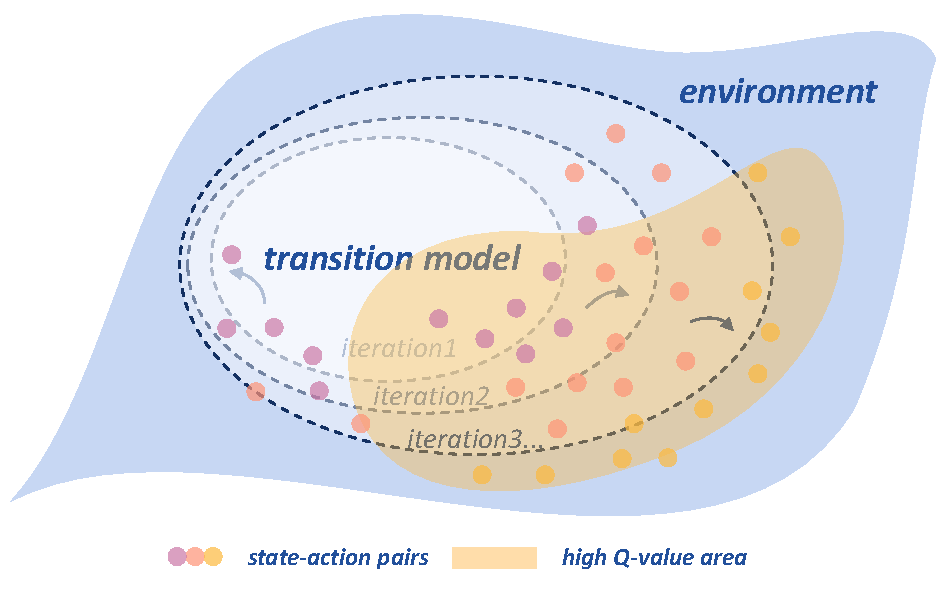
\includegraphics[width=0.6\textwidth]{figures/concept.pdf}
  \caption{基于定向探索模型的离线到在线强化学习算法框架。离线阶段利用不确定性惩罚保守更新策略；在线阶段利用不确定性引导定向探索，采集的样本用于更新转移模型和策略。}
  \label{Fig:Chap4_framework}
\end{figure}


\subsection{离线预训练阶段}\label{Sec4.2.1}

离线预训练阶段的目标是从静态数据集$\mathcal{D}_{off} = \{(s_i, a_i, s_i', r_i)\}_{i=1}^N$中学习环境动力学模型和初始策略。该阶段包含两个核心组件：集成转移模型的训练和基于不确定性惩罚的策略优化。

集成转移模型由$N$个独立训练的神经网络组成，每个网络$\hat{T}_\phi^i$以状态-动作对$(s,a)$为输入，输出下一状态和奖励的联合高斯分布：
\begin{equation}\label{Eq:Chap4_ensemble_model}
  \hat{T}_\phi^i(s', r|s, a) = \mathcal{N}(\mu_\phi^i(s, a), \Sigma_\phi^i(s, a)), \quad i = 1, \ldots, N
\end{equation}

其中$\mu_\phi^i(s, a) \in \mathbb{R}^{d_s + 1}$为预测均值向量，$\Sigma_\phi^i(s, a) \in \mathbb{R}^{(d_s+1) \times (d_s+1)}$为预测协方差矩阵，$d_s$为状态空间维度。各模型采用相同的网络结构但不同的随机初始化，通过最大化离线数据的对数似然独立训练：
\begin{equation}\label{Eq:Chap4_model_training}
  \mathcal{L}(\phi^i) = -\mathbb{E}_{(s,a,s',r) \sim \mathcal{D}_{off}}[\log \hat{T}_\phi^i(s', r|s, a)]
\end{equation}

集成模型的优势在于：一方面，多模型的平均预测可降低单一模型的偏差；另一方面，模型间预测的分歧度可用于量化认知不确定性，为后续的探索引导提供依据。

在策略优化方面，离线阶段采用基于不确定性惩罚的保守更新策略，遵循MOPO\cite{Yu2020MOPO}的框架。具体而言，定义离线阶段的不确定性估计为集成模型预测方差的最大值：
\begin{equation}\label{Eq:Chap4_offline_uncertainty}
  u_{off}(s, a) = \max_{i=1,\ldots,N} \|\Sigma_\phi^i(s, a)\|_F
\end{equation}

其中$\|\cdot\|_F$表示Frobenius范数。该度量捕捉了集成模型中最不确定的预测，反映状态-动作对$(s,a)$处环境动力学的偶然不确定性。基于此，定义不确定性惩罚奖励：
\begin{equation}\label{Eq:Chap4_penalized_reward}
  \tilde{r}(s, a) = \hat{r}(s, a) - \lambda_{off} \cdot u_{off}(s, a)
\end{equation}

其中$\hat{r}(s, a)$为转移模型预测的奖励均值，$\lambda_{off}$为惩罚系数。通过惩罚高不确定性区域的奖励，策略被约束在模型预测可靠的区域内优化，避免外推误差导致的性能退化。

策略优化采用Soft Actor-Critic（SAC）\cite{Haarnoja2018SAC}算法。SAC维护策略网络$\pi_\varphi$和两个Q值网络$Q_{\theta_1}, Q_{\theta_2}$，通过最大化带熵正则的期望回报优化策略：
\begin{equation}\label{Eq:Chap4_sac_objective}
  J(\varphi) = \mathbb{E}_{s \sim \mathcal{D}, a \sim \pi_\varphi}[Q_\theta(s, a) - \alpha \log \pi_\varphi(a|s)]
\end{equation}

其中$\alpha$为温度参数，控制探索与利用的平衡。Q值网络通过最小化时序差分误差更新：
\begin{equation}\label{Eq:Chap4_q_update}
  \mathcal{L}(\theta) = \mathbb{E}_{(s,a,\tilde{r},s') \sim \mathcal{D}}\left[(Q_\theta(s, a) - \tilde{r} - \gamma \mathbb{E}_{a' \sim \pi_\varphi}[\min_{j=1,2} Q_{\bar{\theta}_j}(s', a') - \alpha \log \pi_\varphi(a'|s')])^2\right]
\end{equation}

其中$\bar{\theta}$为目标网络参数。训练数据从离线数据集$\mathcal{D}_{off}$和模型生成数据集$\mathcal{D}_{model}$中按比例采样。模型生成数据通过从离线数据集中采样初始状态，利用当前策略与转移模型交互生成短期轨迹（rollout）获得。

离线预训练阶段完成后，获得初始策略$\pi_{off}$、集成转移模型$\{\hat{T}_\phi^i\}_{i=1}^N$以及Q值网络$Q_\theta$，为在线微调阶段提供基础。


\subsection{在线定向探索阶段}\label{Sec4.2.2}

在线微调阶段的核心目标是通过与真实环境的有限交互，采集高信息量样本以提升策略性能。与传统方法被动采样不同，本文提出的定向探索策略显式引导策略探索高不确定性且高价值的区域。

定向探索的核心思想是在策略优化目标中同时考虑不确定性和动作价值。具体而言，定义在线阶段的探索策略$\pi_\varphi$通过以下目标更新：
\begin{equation}\label{Eq:Chap4_exploration_objective}
  \nabla_\varphi J_\pi(\varphi) = \mathbb{E}_{(s,a) \sim \mathcal{D}_{on}}\left[\nabla_\varphi \log \pi_\varphi(a|s) \cdot (c \cdot u_{on}(s, a) + Q(s, a))\right]
\end{equation}

其中$u_{on}(s, a)$为在线阶段的不确定性估计（详见第\ref{Sec4.4}节），$Q(s, a)$为动作价值函数，$c$为平衡不确定性与价值的权重系数，$\mathcal{D}_{on}$为在线交互采集的数据集。

该目标函数的设计体现了定向探索的双重考量：

第一，不确定性项$u_{on}(s, a)$引导策略探索转移模型覆盖不足的区域。在这些高不确定性区域采集的样本对转移模型的改进贡献最大，可有效扩展模型的有效覆盖范围。从主动学习（Active Learning）的角度，这相当于选择模型最不确定的样本进行标注，是一种高效的数据收集策略。

第二，价值项$Q(s, a)$确保探索集中在高回报区域。单纯追求高不确定性可能导致策略探索与任务目标无关的状态-动作空间，造成在线交互资源的浪费。通过引入价值项，探索被引导至对策略优化有直接贡献的区域，实现探索效率与优化效果的平衡。

在线微调阶段的完整流程如下：

（1）与真实环境交互，使用当前探索策略$\pi_\varphi$采集轨迹数据，存入在线数据集$\mathcal{D}_{on}$。

（2）将在线数据与离线数据合并，更新集成转移模型$\{\hat{T}_\phi^i\}_{i=1}^N$。模型更新采用增量学习方式，在原有参数基础上继续训练，避免遗忘离线阶段学习的动力学知识。

（3）利用更新后的转移模型生成虚拟轨迹，结合真实数据更新Q值网络和策略网络。策略更新同时考虑标准SAC目标和定向探索目标。

（4）根据在线训练进度动态调整不确定性权重$c$（详见第\ref{Sec4.3.2}节），平衡探索与利用。

（5）重复上述步骤直至达到预设的在线交互预算或策略性能收敛。

通过上述迭代过程，转移模型逐步覆盖更广泛的状态-动作空间，策略在真实环境动力学下持续优化，最终实现高效的离线到在线迁移。


\section{不确定性估计与动态权重自适应}\label{Sec4.3}

不确定性估计是定向探索策略的核心组件。本节首先介绍离线和在线阶段采用的差异化不确定性估计方法，随后阐述动态权重自适应机制。


\subsection{双重不确定性估计}\label{Sec4.3.1}

如第二章所述，强化学习中的不确定性可分为偶然不确定性和认知不确定性两类。偶然不确定性源于环境固有的随机性，无法通过收集更多数据消除；认知不确定性源于模型对环境知识的缺乏，可通过在线探索逐步降低。在离线和在线两个阶段，两类不确定性的作用有所不同，因此本文采用差异化的不确定性估计方法。

在离线阶段，由于无法与真实环境交互，认知不确定性无法降低，因此主要关注偶然不确定性。偶然不确定性通过集成模型的预测方差估计：
\begin{equation}\label{Eq:Chap4_aleatoric_uncertainty}
  u_{off}(s, a) = \max_{i=1,\ldots,N} \|\Sigma_\phi^i(s, a)\|_F
\end{equation}

该度量反映环境动力学在状态-动作对$(s,a)$处的内在随机性。取集成模型中的最大方差是一种保守估计，确保在任一模型预测不确定时都施加惩罚。

在在线阶段，目标是主动探索高认知不确定性区域以补充转移模型。因此，除偶然不确定性外，还需捕捉认知不确定性。认知不确定性通过集成模型均值预测的分歧度估计：
\begin{equation}\label{Eq:Chap4_epistemic_uncertainty}
  \text{DisVar}(s, a) = \frac{1}{d}\sum_{j=1}^{d} \text{Var}_{i=1,\ldots,N}[\mu_{\phi,j}^i(s, a)]
\end{equation}

其中$d$为预测向量维度，$\mu_{\phi,j}^i(s, a)$为第$i$个模型预测均值的第$j$个分量，$\text{Var}_{i=1,\ldots,N}[\cdot]$表示在集成成员间计算方差。该度量的核心思想是：在数据充分覆盖的区域，各模型因接收到足够的监督信号而收敛至相近的预测，分歧度较低；在数据稀疏的区域，模型因初始化差异而产生显著不同的预测，分歧度较高。

在线阶段的不确定性估计综合两类不确定性：
\begin{equation}\label{Eq:Chap4_online_uncertainty}
  u_{on}(s, a) = \max_{i=1,\ldots,N} \|\Sigma_\phi^i(s, a)\|_F + \sqrt{\text{DisVar}(s, a)}
\end{equation}

第一项为偶然不确定性，第二项为认知不确定性的标准差形式。两项相加确保探索策略同时考虑环境的内在随机性和模型的知识缺乏，引导策略探索模型预测最不可靠的区域。


\subsection{动态权重自适应机制}\label{Sec4.3.2}

在定向探索目标（公式\ref{Eq:Chap4_exploration_objective}）中，权重系数$c$控制不确定性与价值的相对重要性。由于不同任务的状态空间和奖励尺度存在显著差异，$Q(s,a)$和$u_{on}(s,a)$的数值量级可能相差悬殊。为便于跨任务调节权重，首先对两项进行归一化处理。

具体而言，在离线阶段计算$\mathbb{E}_{(s,a) \sim \mathcal{D}_{off}}[Q(s,a)]$和$\mathbb{E}_{(s,a) \sim \mathcal{D}_{off}}[u(s,a)]$的均值和标准差。在线阶段，对计算得到的$Q(s,a)$和$u_{on}(s,a)$进行标准化：
\begin{equation}\label{Eq:Chap4_normalization}
  \bar{Q}(s,a) = \frac{Q(s,a) - \mu_Q}{\sigma_Q}, \quad \bar{u}_{on}(s,a) = \frac{u_{on}(s,a) - \mu_u}{\sigma_u}
\end{equation}

其中$\mu_Q, \sigma_Q$和$\mu_u, \sigma_u$分别为离线阶段统计得到的均值和标准差。归一化后，两项处于可比较的数值范围，权重$c$的调节更加直观。

此外，在在线微调过程中，不确定性与价值的相对重要性应随训练进度动态调整。在训练初期，模型覆盖范围有限，应优先探索高不确定性区域以扩展模型的有效范围；在训练后期，模型已较为完善，应转向利用已学习的知识优化策略，即更多关注高价值区域。

为实现上述动态平衡，本文采用Sigmoid函数调制权重$c$随策略更新步数$k$的衰减：
\begin{equation}\label{Eq:Chap4_dynamic_weight}
  c = c_0 \cdot \frac{1}{1 + e^{(k - k_0) \cdot \nu}}
\end{equation}

其中$c_0$为初始权重，$k_0$为衰减中心点，$\nu$为衰减速率。该函数具有以下特性：当$k < k_0$时，$c$接近$c_0$，策略重视不确定性引导的探索；当$k > k_0$时，$c$逐渐衰减至接近0，策略转向价值引导的利用；衰减过程平滑连续，避免策略行为的突变。

通过动态权重自适应机制，算法在训练初期充分探索以补充转移模型，在训练后期充分利用以优化策略性能，实现探索与利用的自适应平衡。


\section{理论分析}\label{Sec4.4}

本节从理论角度分析定向探索策略相比均匀采样的优势。核心结论是：在转移函数满足分段常数假设的条件下，基于不确定性引导的定向探索可实现更优的模型收敛速率。

在实际应用中，许多物理系统的动力学具有分段常数特性。例如，机器人控制任务中，不同操作模式（如空载与负载）对应不同的动力学参数；自动驾驶场景中，不同路面条件（如干燥与湿滑）导致车辆响应特性的显著差异。这些场景的转移函数可近似为在不同状态-动作区域内取不同常数值的分段常数函数。

\begin{defn}[分段常数函数]\label{Def:Chap4_piecewise_constant}
  设$\mathcal{X} \subset \mathbb{R}^d$为状态-动作空间的子集。函数$T: \mathcal{X} \rightarrow \mathbb{R}$称为分段常数函数，若存在$\mathcal{X}$的有限划分$\{R_1, \ldots, R_M\}$，使得$T$在每个区域$R_m$内取常数值$c_m$。记$\text{PC}(\beta, M)$为满足$\sum_{m=1}^{M}|\partial R_m|^\beta < \infty$的分段常数函数集合，其中$|\partial R_m|$表示区域$R_m$边界的测度，$\beta$为边界平滑性参数。
\end{defn}

基于上述定义，可建立定向探索策略的收敛速率下界。

\begin{thm}[定向探索的收敛速率]\label{Thm:Chap4_convergence}
  设转移函数$T \in \text{PC}(\beta, M)$为分段常数函数，$\hat{T}$为基于在线数据集$\mathcal{D}_{on}$学习得到的转移模型估计。若采样策略基于不确定性引导，即优先采样模型预测方差最大的状态-动作对，则模型估计误差的下界为：
  \begin{equation}\label{Eq:Chap4_convergence_bound}
    \inf_{\hat{T}} \sup_{T \in \text{PC}(\beta, M)} \mathbb{E}[\|\hat{T} - T\|^2] \geq c \cdot |\mathcal{D}_{on}|^{-\frac{1}{d-1}}
  \end{equation}
  其中$c > 0$为与区域复杂度相关的常数，$d$为状态-动作空间的内在维度，$|\mathcal{D}_{on}|$为在线数据集的样本数量。
\end{thm}

\begin{proof}
  该定理的证明基于主动学习理论中的经典结果\cite{Willett2005Faster}。核心思想是：对于分段常数函数，估计误差主要来源于函数不连续点（区域边界）附近的不确定性。基于不确定性引导的采样策略优先在这些边界区域采集样本，从而更高效地定位不连续点，降低估计误差。详细证明参见文献\cite{Willett2005Faster}中定理2的推导。
\end{proof}

作为对比，均匀采样策略的收敛速率下界为\cite{Korostelev1999Minimax}：
\begin{equation}\label{Eq:Chap4_uniform_bound}
  \inf_{\hat{T}} \sup_{T \in \text{PC}(\beta, M)} \mathbb{E}[\|\hat{T} - T\|^2] \geq c' \cdot |\mathcal{D}_{on}|^{-\frac{1}{d}}
\end{equation}

比较公式\ref{Eq:Chap4_convergence_bound}和公式\ref{Eq:Chap4_uniform_bound}，定向探索策略的收敛速率指数为$-\frac{1}{d-1}$，优于均匀采样的$-\frac{1}{d}$。这意味着在相同样本数量下，定向探索可实现更低的模型估计误差；或者，达到相同精度所需的样本数量更少。该理论结果为本文算法的样本效率优势提供了理论支撑。

需要指出的是，上述理论分析基于分段常数函数的假设，而实际环境的转移函数可能更为复杂。然而，分段常数函数可视为对复杂函数的局部近似，该理论结果仍具有指导意义：基于不确定性引导的定向探索在函数变化剧烈（对应高不确定性）的区域采集更多样本，有助于更精确地刻画转移函数的复杂结构。


\section{算法流程}\label{Sec4.5}

综合以上各节内容，本文提出的基于定向探索模型的离线到在线强化学习算法的完整流程如算法\ref{Alg:Chap4_DEM}所示。

\begin{algorithm}[htbp]
  \caption{基于定向探索模型的离线到在线强化学习算法}
  \label{Alg:Chap4_DEM}
  \begin{algorithmic}[1]
    \Require 离线数据集$\mathcal{D}_{off}$，集成模型数量$N$，离线训练轮数$E_{off}$，在线交互轮数$E_{on}$，初始探索权重$c_0$，衰减参数$k_0, \nu$，惩罚系数$\lambda_{off}$
    \Ensure 优化后的策略$\pi_\varphi$
    \State // 离线预训练阶段
    \State 初始化集成转移模型$\{\hat{T}_\phi^i\}_{i=1}^N$、策略网络$\pi_\varphi$、Q值网络$Q_{\theta_1}, Q_{\theta_2}$
    \For{$e = 1$ to $E_{off}$}
    \State 在$\mathcal{D}_{off}$上训练集成转移模型（公式\ref{Eq:Chap4_model_training}）
    \State 利用转移模型生成虚拟轨迹，存入$\mathcal{D}_{model}$
    \State 计算不确定性惩罚奖励$\tilde{r}$（公式\ref{Eq:Chap4_penalized_reward}）
    \State 从$\mathcal{D}_{off} \cup \mathcal{D}_{model}$采样，更新Q值网络和策略网络
    \EndFor
    \State 统计$\mathcal{D}_{off}$上$Q(s,a)$和$u(s,a)$的均值和标准差
    \State // 在线微调阶段
    \State 初始化在线数据集$\mathcal{D}_{on} \leftarrow \emptyset$
    \For{$e = 1$ to $E_{on}$}
    \State 使用策略$\pi_\varphi$与真实环境交互，采集轨迹数据加入$\mathcal{D}_{on}$
    \State 合并$\mathcal{D}_{off}$和$\mathcal{D}_{on}$，更新集成转移模型
    \State 计算在线不确定性$u_{on}(s,a)$（公式\ref{Eq:Chap4_online_uncertainty}）
    \State 更新动态权重$c$（公式\ref{Eq:Chap4_dynamic_weight}）
    \State 利用定向探索目标更新策略（公式\ref{Eq:Chap4_exploration_objective}）
    \State 更新Q值网络
    \EndFor
    \State \Return 策略$\pi_\varphi$
  \end{algorithmic}
\end{algorithm}

算法的时间复杂度主要由以下部分组成：（1）集成模型训练，复杂度为$O(N \cdot |\mathcal{D}| \cdot d_{model})$，其中$d_{model}$为模型参数量；（2）不确定性估计，复杂度为$O(N \cdot d)$，其中$d$为预测向量维度；（3）策略和Q值网络更新，与标准SAC相同。由于集成模型可并行训练，实际计算开销与单模型方法相当。

算法的空间复杂度主要由集成模型参数和经验回放池占用。集成模型的参数量为$O(N \cdot d_{model})$，经验回放池的存储需求与数据集大小成正比。在实际实现中，$N$通常取5-7，不会显著增加存储开销。


\section{实验验证}\label{Sec4.7}

本节通过在D4RL基准测试集上的实验验证本文算法的有效性。实验设计旨在回答以下问题：（1）本文算法与现有离线到在线强化学习方法及基于模型的离线强化学习方法相比表现如何？（2）基于不确定性引导的定向探索是否确实聚焦于高不确定性、高价值区域？（3）动态权重自适应机制对最终性能的贡献如何？


\subsection{实验设置}\label{Sec4.7.1}

本节介绍实验所采用的数据集、实现细节和基线方法。

在数据集选择方面，本文在D4RL基准测试集\cite{Fu2020D4RL}上评估算法性能。D4RL是基于MuJoCo物理仿真器\cite{Todorov2012MuJoCo}构建的离线强化学习标准评测平台，包含多种环境和数据集类型。本文选取三种连续控制环境（halfcheetah、hopper、walker2d）和三种数据集类型（medium、medium-replay、medium-expert），共计9个问题设置。所有数据集均采用v2版本，具体组成如下：（1）medium数据集包含由提前终止的SAC策略生成的转移样本，代表中等质量的离线数据；（2）medium-replay数据集由训练medium策略过程中的经验回放池组成，包含从随机策略到中等策略的完整训练轨迹；（3）medium-expert数据集混合了次优策略和专家策略的数据，代表高质量但分布不均匀的离线数据。

在实验实现方面，本文遵循SAC\cite{Haarnoja2018SAC}和MOPO\cite{Yu2020MOPO}的基本超参数设置。需要调整的超参数主要包括模型生成轨迹的长度$h$和惩罚系数$\lambda_{off}$。所有任务均在3个随机种子上运行。在线交互阶段，每轮交互采集50k步样本，权重调整速率$\nu$设为0.001，衰减中心点$k_0$设为5000。为保证公平性和一致性，策略训练总步数设为1M步，每1k步评估一次策略性能。

在基线方法方面，本文与以下算法进行对比：离线到在线强化学习算法AWAC\cite{Nair2020AWAC}；基于模型的离线强化学习算法MOPO\cite{Yu2020MOPO}、COMBO\cite{Yu2021COMBO}和MOREL\cite{Kidambi2020MOReL}；经典离线强化学习算法CQL\cite{Kumar2020CQL}和TD3+BC\cite{Fujimoto2021TD3BC}。由于本文算法建立在MOPO基础上并增加在线微调过程，与MOPO的对比可视为消融研究。所有基线方法的结果均引用自原始论文。


\subsection{实验结果}\label{Sec4.7.2}

表\ref{Tab:Chap4_Performance}展示了本文算法与基线方法在D4RL基准测试集上的性能对比。实验结果报告为最后10次评估的平均归一化得分，$\pm$表示3个随机种子的标准差。得分采用D4RL标准归一化程序\cite{Fu2020D4RL}，归一化至0到100的范围，其中0分对应随机策略，100分对应专家策略。

\begin{table}[htbp]
  \centering
  \caption{D4RL基准测试集上的性能对比}
  \label{Tab:Chap4_Performance}
  \resizebox{\textwidth}{!}{
    \begin{tabular}{llrrrrrrr}
      \toprule
      数据集类型         & 环境          & 本文算法                     & MOPO & COMBO & AWAC  & MOREL & CQL   & TD3+BC           \\
      \midrule
      medium        & halfcheetah & $\mathbf{70.5 \pm 4.2}$  & 42.3 & 54.2  & 41.1  & 42.1  & 44.4  & 42.8             \\
                    & hopper      & $65.5 \pm 10.9$          & 28.0 & 97.2  & 91.0  & 95.4  & 86.6  & $\mathbf{99.5}$  \\
                    & walker2d    & $\mathbf{86.6 \pm 0.5}$  & 17.8 & 81.9  & 79.1  & 77.8  & 74.5  & 79.7             \\
      \midrule
      medium-replay & halfcheetah & $\mathbf{73.1 \pm 0.4}$  & 53.1 & 55.1  & -     & 40.2  & 46.2  & 43.3             \\
                    & hopper      & $\mathbf{96.1 \pm 5.9}$  & 67.5 & 89.5  & -     & 93.6  & 48.6  & 31.4             \\
                    & walker2d    & $\mathbf{82.6 \pm 0.3}$  & 39.0 & 56.0  & -     & 49.8  & 32.6  & 25.2             \\
      \midrule
      medium-expert & halfcheetah & $75.4 \pm 13.3$          & 63.3 & 90.0  & 41.0  & 53.3  & 62.4  & $\mathbf{97.9}$  \\
                    & hopper      & $102.2 \pm 0.8$          & 23.7 & 111.1 & 111.9 & 108.7 & 111.0 & $\mathbf{112.2}$ \\
                    & walker2d    & $\mathbf{111.4 \pm 0.4}$ & 44.6 & 103.3 & 78.3  & 95.6  & 98.7  & 101.1            \\
      \bottomrule
    \end{tabular}
  }
\end{table}

从表\ref{Tab:Chap4_Performance}可以看出，本文算法在多数任务上取得了优异的性能表现。在medium-replay数据集的全部三个环境中，本文算法均取得最高得分，显著优于所有基线方法。这一结果表明，当离线数据质量参差不齐时，本文的定向探索策略能够有效识别并补充高价值区域的样本，显著提升策略性能。

值得注意的是，本文算法在所有9个问题设置上均优于MOPO算法，验证了在线微调框架的有效性。考虑到本文仅使用50k步的在线交互量，远低于传统离线到在线强化学习算法所需的200k步以上，这一结果尤为突出。

然而，本文算法在medium-expert数据集上的表现相对较弱。分析其原因在于：medium-expert数据集的离线数据高度集中在高奖励区域，导致期望奖励高但不确定性低。这种数据分布限制了在线交互阶段采集的数据多样性和质量，进而约束了算法的提升空间。相比之下，基于行为克隆的强化学习方法（如TD3+BC）在高质量数据集上表现优异，这为后续改进提供了思路：引入行为克隆损失项可能有助于提升算法在此类环境中的性能。


\subsection{模型覆盖范围的可视化验证}\label{Sec4.7.3}

为验证基于不确定性引导的定向探索是否确实聚焦于高期望回报和高不确定性区域，本节进行可视化实验分析。具体而言，选取三种不同类型的数据集进行可视化：hopper-medium、hopper-medium-replay和hopper-medium-expert。

实验过程如下：首先，从离线数据集中采样2000个转移样本$(s, a, s', r)$；然后，将离线状态$s$输入转移模型，获得模型预测的转移样本$(s, a_T, s'_T, r_T)$；接着，使用t-SNE算法\cite{vanderMaaten2008tSNE}将$\{s'\}$和$\{s'_T\}$投影至二维平面；最后，绘制$\{s'_T\}$的散点图，使用离线策略的Q值网络估计状态-动作对$(s, a_T)$的期望回报，并将Q值映射为散点颜色。同时，显示离线状态$\{s'\}$的核密度估计作为参照。可视化结果如图\ref{Fig:Chap4_tsne}所示。

\begin{figure}[htbp]
  \centering
  
\includegraphics[width=1\textwidth]{figures/tsne.pdf}
  \caption{模型预测状态与离线数据的对比。将模型预测状态和离线状态数据密度在三种不同离线数据集上进行可视化。散点表示模型的数据分布，预测Q值经归一化后作为散点的颜色。}
  \label{Fig:Chap4_tsne}
\end{figure}

从图\ref{Fig:Chap4_tsne}可以观察到，模型预测的状态主要分布在低密度的边缘区域，且散点大多呈现红色，表明这些区域具有高不确定性和高期望回报。这一现象表明，在策略引导下，模型确实更多地关注高不确定性且高动作价值的区域。

对比三个子图可以发现：在hopper-medium-replay环境中，散点分布较为分散，表明在线交互实现了充分的探索，补充了更多分布外数据；在hopper-medium-expert环境中，散点分布更为集中，这是因为专家数据的高质量和低方差使得在线交互难以通过探索采集到更高动作价值的数据，导致补充的数据质量可能不及离线数据集中的专家数据，模型更新不够充分。这一观察结果进一步印证了本文算法更适用于数据分布均匀的环境，而在高质量数据集上的适用性有限。


\subsection{动态权重自适应的消融实验}\label{Sec4.7.4}

为验证动态权重自适应机制的有效性，本节设计消融实验，将完整算法与移除动态权重自适应的变体（记为DEM-s）进行对比。DEM-s中，不确定性权重参数$c$固定为初始值$c_0$，不随在线交互步数增加而衰减。其余超参数与主实验保持一致。

\begin{table}[htbp]
  \centering
  \caption{动态权重自适应的消融实验结果}
  \label{Tab:Chap4_ablation}
  \begin{tabular}{llrr}
    \toprule
    数据集类型         & 环境          & 本文算法            & 无动态权重            \\
    \midrule
    medium        & halfcheetah & $\mathbf{70.5}$ & $64.7$           \\
                  & hopper      & $\mathbf{65.5}$ & $53.0$           \\
                  & walker2d    & $\mathbf{86.6}$ & $86.2$           \\
    \midrule
    medium-replay & halfcheetah & $\mathbf{73.1}$ & $72.6$           \\
                  & hopper      & $\mathbf{96.1}$ & $90.2$           \\
                  & walker2d    & $\mathbf{82.6}$ & $82.1$           \\
    \midrule
    medium-expert & halfcheetah & $\mathbf{75.4}$ & $36.1$           \\
                  & hopper      & $102.2$         & $102.2$          \\
                  & walker2d    & $111.4$         & $\mathbf{112.0}$ \\
    \bottomrule
  \end{tabular}
\end{table}

表\ref{Tab:Chap4_ablation}展示了消融实验结果。完整算法在几乎所有任务上均取得更优性能，尤其在hopper-medium和halfcheetah-medium-expert任务上提升显著：完整算法分别取得65.5和75.4的得分，而无动态权重变体仅为53.0和36.1。然而，在walker2d-medium-expert任务上，完整算法略低于无动态权重变体，推测这与该任务高度结构化的专家数据有关，早期探索阶段可能对策略产生轻微干扰。

上述结果表明，动态权重自适应机制在平衡探索与利用方面发挥了关键作用。在交互初期，较高的不确定性权重鼓励探索，使策略覆盖更广泛的状态-动作空间；随着交互推进，权重逐渐降低，使算法聚焦于高奖励区域并稳定策略性能。这种自适应机制使算法能够根据训练进度动态调整探索-利用平衡，优于固定权重的静态策略。


\section{本章小结}\label{Sec4.8}

本章详细介绍了基于定向探索模型的离线到在线强化学习算法。首先分析了现有方法在保守性与灵活性、不确定性利用、在线交互成本等方面的局限，阐明了将不确定性从惩罚信号转变为探索引导信号的核心思想。随后系统阐述了算法的两阶段框架：离线阶段通过集成模型和不确定性惩罚进行保守策略优化；在线阶段通过定向探索目标引导策略探索高不确定性且高价值的区域，以最少的在线交互实现高效微调。

在技术实现层面，本章介绍了双重不确定性估计方法，区分偶然不确定性和认知不确定性在不同阶段的作用；提出了动态权重自适应机制，通过Sigmoid函数实现探索与利用的平滑过渡。在理论分析层面，证明了在分段常数函数假设下，定向探索策略相比均匀采样具有更优的收敛速率，为算法的样本效率优势提供了理论支撑。

在实验验证层面，本章在D4RL基准测试集的9个问题设置上进行了系统评估。实验结果表明：（1）本文算法在medium-replay数据集上显著优于所有基线方法，在所有任务上均优于MOPO；（2）通过t-SNE可视化验证了定向探索确实聚焦于高不确定性、高价值区域；（3）消融实验证明了动态权重自适应机制对最终性能的积极贡献。实验同时揭示了算法在high-quality数据集上的局限性，为后续改进指明了方向。
